%% 
%% Copyright 2007, 2008, 2009 Elsevier Ltd
%% 
%% This file is part of the 'Elsarticle Bundle'.
%% ---------------------------------------------
%% 
%% It may be distributed under the conditions of the LaTeX Project Public
%% License, either version 1.2 of this license or (at your option) any
%% later version.  The latest version of this license is in
%%    http://www.latex-project.org/lppl.txt
%% and version 1.2 or later is part of all distributions of LaTeX
%% version 1999/12/01 or later.
%% 
%% The list of all files belonging to the 'Elsarticle Bundle' is
%% given in the file `manifest.txt'.
%% 
%% Template article for Elsevier's document class `elsarticle'
%% with harvard style bibliographic references
%% SP 2008/03/01

\documentclass[preprint,12pt,authoryear]{elsarticle}

%% Use the option review to obtain double line spacing
%% \documentclass[authoryear,preprint,review,12pt]{elsarticle}

%% Use the options 1p,twocolumn; 3p; 3p,twocolumn; 5p; or 5p,twocolumn
%% for a journal layout:
%% \documentclass[final,1p,times,authoryear]{elsarticle}
%% \documentclass[final,1p,times,twocolumn,authoryear]{elsarticle}
%% \documentclass[final,3p,times,authoryear]{elsarticle}
%% \documentclass[final,3p,times,twocolumn,authoryear]{elsarticle}
%% \documentclass[final,5p,times,authoryear]{elsarticle}
%% \documentclass[final,5p,times,twocolumn,authoryear]{elsarticle}

%% For including figures, graphicx.sty has been loaded in
%% elsarticle.cls. If you prefer to use the old commands
%% please give \usepackage{epsfig}

%% The amssymb package provides various useful mathematical symbols
\usepackage{amssymb}
\usepackage{amsmath}
\usepackage{color, soul}
\usepackage{url}
\usepackage{booktabs}
\usepackage{longtable}
\usepackage{pdflscape}
%% The amsthm package provides extended theorem environments
%% \usepackage{amsthm}

%% The lineno packages adds line numbers. Start line numbering with
%% \begin{linenumbers}, end it with \end{linenumbers}. Or switch it on
%% for the whole article with \linenumbers.
\usepackage{lineno}

%% Block of code for fixing corresponding author bug 
%% in elsarticle template... Don't really understand it
\makeatletter
\def\@author#1{\g@addto@macro\elsauthors{\normalsize%
    \def\baselinestretch{1}%
    \upshape\authorsep#1\unskip\textsuperscript{%
      \ifx\@fnmark\@empty\else\unskip\sep\@fnmark\let\sep=,\fi
      \ifx\@corref\@empty\else\unskip\sep\@corref\let\sep=,\fi
      }%
    \def\authorsep{\unskip,\space}%
    \global\let\@fnmark\@empty
    \global\let\@corref\@empty  %% Added
    \global\let\sep\@empty}%
    \@eadauthor={#1}
}
\makeatother
%% End block of weird code


%% Command for bold Greek symbols
\newcommand{\mitbf}[1]{\hbox{\mathversion{bold}$#1$}}

\journal{Earth and Planetary Science Letters}

\begin{document}

\begin{frontmatter}

%% Title, authors and addresses

%% use the tnoteref command within \title for footnotes;
%% use the tnotetext command for theassociated footnote;
%% use the fnref command within \author or \address for footnotes;
%% use the fntext command for theassociated footnote;
%% use the corref command within \author for corresponding author footnotes;
%% use the cortext command for theassociated footnote;
%% use the ead command for the email address,
%% and the form \ead[url] for the home page:
%% \title{Title\tnoteref{label1}}
%% \tnotetext[label1]{}
%% \author{Name\corref{cor1}\fnref{label2}}
%% \ead{email address}
%% \ead[url]{home page}
%% \fntext[label2]{}
%% \cortext[cor1]{}
%% \address{Address\fnref{label3}}
%% \fntext[label3]{}

\title{Bayesian inversion for paleomagnetic reconstruction and plate kinematics}

%% use optional labels to link authors explicitly to addresses:
%% \author[label1,label2]{}
%% \address[label1]{}
%% \address[label2]{}

\author{Ian Rose\corref{cor1}\fnref{ref1}}
\author{Bruce Buffett\fnref{ref1}}
\author{Nicholas Swanson-Hysell\fnref{ref1}}

\fntext[ref1]{University of California, Berkeley}
\cortext[cor1]{Corresponding author, \url{ian.rose@berkeley.edu}}

\address{}

\begin{abstract}
Apparent polar wander (APW) paths from paleomagnetic poles provide the most direct data
for reconstructing past paleogeography and plate motions for times earlier than $\sim$200 Ma. 
However, it has proven difficult to interpret APW paths in the presence of large errors,
age uncertainties, and the lack of paleolongitude control in traditional paleomagnetic analysis.
Approaches for dealing with the uncertainties in APW paths include spline fits and running means.
Here we propose a new approach for interpretation of APW paths.
It extends the paleomagnetic Euler pole analysis of \citet{gordon1984paleomagnetic}
by placing it within the framework of a Bayesian inverse problem.
This allows the natural incorporation of uncertainties in both pole position and age.
The resulting paleomagnetic Euler poles provide estimates for the total
plate motions (not just the latitudinal components) as well as their uncertainties.

We show several example inversions on synthetic data to demonstrate the capabilities of the method.
We also show examples using real paleomagnetic data from Australia and 
from the Laurentian Keweenawan province. The latter inversion gives a plate
speed for Mesoproterozoic Laurentia of between 22.9 and 39.1 cm/yr for a 95\% credible interval.
\end{abstract}

\begin{keyword}
%% keywords here, in the form: keyword \sep keyword

%% PACS codes here, in the form: \PACS code \sep code

%% MSC codes here, in the form: \MSC code \sep code
%% or \MSC[2008] code \sep code (2000 is the default)

\end{keyword}

\end{frontmatter}

\linenumbers

%% main text
\section{Introduction}
\label{sec:introduction}

Plate tectonics is the motion of near-rigid blocks of lithosphere across the surface of Earth, 
separated by narrow regions of deformation in spreading centers, transform faults, and subduction zones.
The rigidity of plates means that the motion of most of Earth's surface
can be described by a set of Euler poles which specify the position and magnitude of the rotation axis for a
given plate \citep[cf.][]{cox2009plate}. Individual points on a plate undergoing
rigid rotation are described by small circle paths.

Euler poles are ubiquitous in describing current plate motions 
\citep[e.g.][]{demets1990current, argus2011geologically} due to their simplicity and compactness.
Furthermore, there are good reasons to think that plate motions remain constant, or approximately
so, over millions to tens of millions of years. This is most dramatically seen in the shape
of oceanic fracture zones and in hotspot tracks across the lithosphere. These features
form gently curving arcs over large portions of Earth's surface which are well described by small
circles, consistent with finite Euler rotations of the plate for an extended period of time.
As such, the combination of an Euler pole plus a time interval through which it rotates 
(often called a ``stage pole'') is a convenient description of plate motions through Earth history.

The stage pole description of plate motions is therefore a convenient way of reconstructing
plate tectonic history, and is widely used in both continental reconstruction 
\citep[e.g.][]{boyden2011next} and in geodynamical
modeling \citep[e.g.][]{mcnamara2005thermochemical, bull2014effect, rudolph2014history}.
Most reconstructions of plate motions rely heavily on fitting Euler pole rotations
to oceanic fracture zones, hotspot tracks, seafloor magnetic isochrons,
and, to a lesser extent, paleomagnetic data \citep{muller1993revised, seton2012global}.
However, as we look further back in Earth history, many of the records on which these
plate tectonic reconstructions rely largely disappear due to the 
subduction of oceanic lithosphere. Before $\sim$200 Ma there is no oceanic record,
and the paleomagnetic record from continental rocks is the dominant remaining evidence.

It is more challenging to reconstruct past plate motions from the paleomagnetic
record for a number of reasons, including 
(1) the data are often sparser,
(2) traditional paleomagnetic analysis constraints paleolatitude and orientation
of the lithosphere but has no way of constraining paleolongitude, and
(3) some paleomagnetic poles have poor age control.

\citet{gordon1984paleomagnetic} noted that apparent polar wander paths (APW paths) have 
arcing trajectories similar to fracture zones and hotspot tracks, which is
to be expected if similar tectonic processes are responsible for creating them.
They therefore suggested fitting small circles to paleomagnetic poles tracks,
which would furnish Euler poles for the plate in question for that time period.
This model for understanding APW paths, called paleomagnetic Euler pole (PEP) analysis,
 had the attractive feature of providing a complete description of the plate motion, 
including paleolongitudinal changes and speeds. 
However, it had the drawback of being somewhat difficult to estimate,
uncertainties in the fit were not easily computed, 
and it did not incorporate age uncertainties. 
A rigorous treatment of the uncertainties requires significant computational effort.
With a few exceptions \citep[e.g.][]{beck1989paleomagnetism, tarling1996palaeomagnetic, bryan1986rotation, beck2003absolute, smirnov2010co},
PEP analysis has not seen wide adoption.

Herein we extend paleomagnetic Euler pole analysis by placing it within
a Bayesian statistical framework, and demonstrate how to invert for PEPs
using Markov Chain Monte Carlo (MCMC) methods. This framework has the advantage
of naturally incorporating uncertainties in the paleomagnetic pole positions,
as well as widely disparate age uncertainties that commonly occur in APW paths.
The resulting stage poles for which we invert are not a single answer, but are instead
a distribution of possible answers, furnishing uncertainties as part of the solution process.
\citet{iaffaldano2012reconstructing} employed a similar approach for recent 
plate motions in trying to reconstruct India's Cenozoic convergence with Asia.

The paper is organized as follows: in Section~\ref{sec:apwp} we review different
approaches for interpreting APW paths. In Section~\ref{sec:bayesian_inversion} we
describe the formalism of Bayesian inversions and Markov Chain Monte Carlo methods.
In Section~\ref{sec:model} we describe the statistical model which we will be inverting.
In Section~\ref{sec:example_inversion} we demonstrate the inversion on several
synthetic data sets. In Sections~\ref{sec:australia} and~\ref{sec:keweenawan}
we show examples using real paleomagnetic data from Australia and Laurentia,
including interpretations of plate speeds.

\section{Interpretation of APW paths}
\label{sec:apwp}
\begin{figure*}
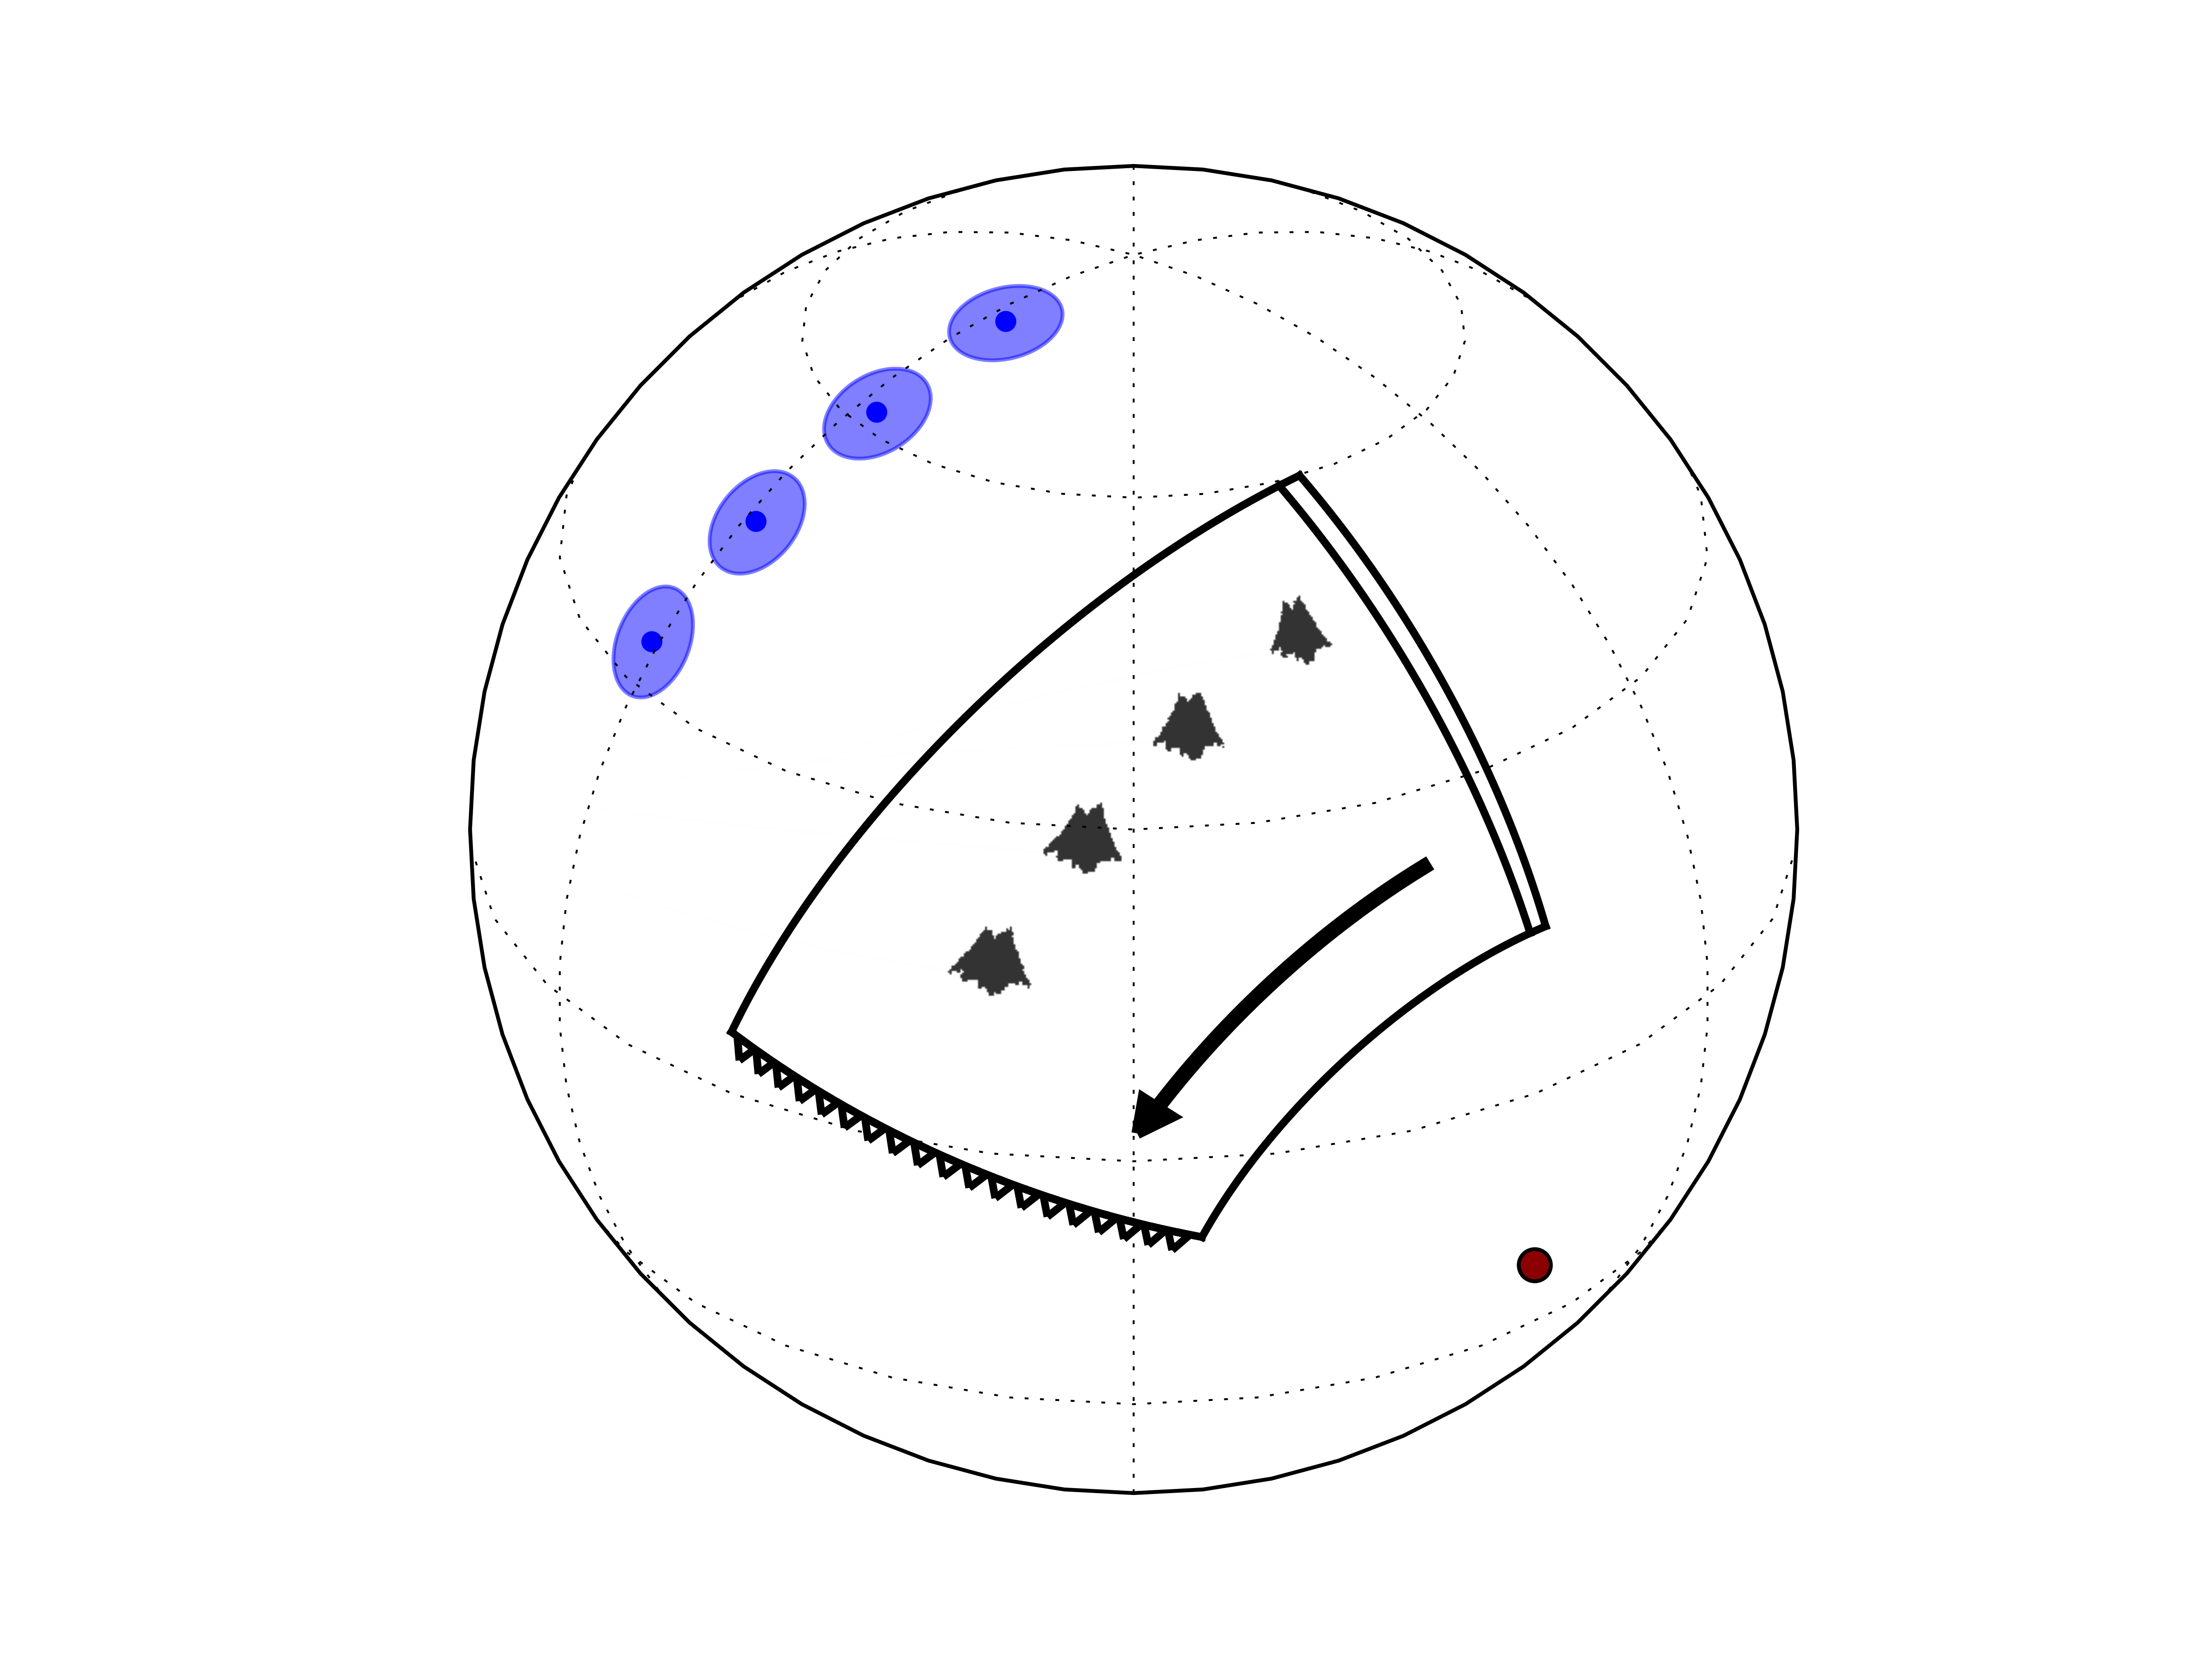
\includegraphics[width=0.9\textwidth]{figures/cartoon/paleomagnetic_euler_pole.png}
\caption[Conceptual model for a paleomagnetic Euler pole.]{Conceptual model for a paleomagnetic Euler pole. A finite rotation of the plate around an Euler pole results in long, arcuate oceanic fracture zones and hotspot tracks which describe small circles on the globe. The same finite rotation produces a small circle in the APW path. By fitting a small circle to the APW path we may recover the Euler pole that produced the rotation. Adapted from \citet{gordon1984paleomagnetic}}
\label{fig:pep}
\end{figure*}
A sequence of paleomagnetic poles from the same continental block form an APW path,
which can then be used to develop plate tectonic reconstructions and models
of plate speeds through time. Interpretation of these paths becomes difficult in the
case of limited or highly uncertain data, and when the age of paleomagnetic poles are poorly
known. A number of approaches to dealing with uncertainty in APW paths have been developed,
which we briefly review here.

\subsection{Latitudinal drift}
\label{sec:latitudinal_drift}
Due to the rotational symmetry of Earth's magnetic field, paleomagnetic poles do not
directly constrain the paleolongitude of the continental block in question \citep{butler1992paleomagnetism}.
The simplest analysis of an APW path is thus to compare the paleolatitudes implied successive poles.
The difference in paleolatitudes gives a mininimum angular distance over which the block has traveled. 
If the two poles are well-dated, this also furnishes a rate of latitudinal motion.

It is also possible to estimate confidence bounds on the rate of latitudinal drift by
bootstrap resampling \citep[e.g.][]{tarduno1990fast} or by taking a Monte Carlo approach. 
\citet{swanson2014confirmation} generated samples from Fisher distributions
for a pair of poles from the Proterozoic Laurentian Midcontinent Rift zone to estimate the range
of implied latitudinal drift rates. They also sampled from the age uncertainties, assuming
Gaussian distributions on the radiometric dates, which incorporated the age uncertainties of the poles.
With pseudosamples of pole position and ages, they were able to estimate the 95\% 
confidence estimates on the rate of latitudinal drift.

Whether using point estimates of the latitudinal drift rate or using Monte Carlo estimates, 
the latitudinal drift interpretation of APW paths remains limited.
It has no control over longitudinal drift rate, 
nor does it naturally extend to APW paths with more than two poles, 
especially if two coeval poles are not in agreement.

\subsection{Spherical splines}
\label{sec:spherical_splines}
When considering APW paths with many poles, it becomes more difficult to perform
latitudinal comparisons between pairs of poles. It is not always clear which pairs of
poles to compare in cases where there are many overlapping paleomagnetic poles,
often of unclear age progression and variable reliabilities.

One approach to deal with these uncertainties is to fit a spline through the
set of paleomagnetic poles, constraining the path to lie on the surface of a sphere.
This approach was pioneered by \citet{torsvik1992baltica} using the spherical spline
algorithm developed by \citet{jupp1987fitting}.
This approach has the advantage of allowing the weighting of the data by their
uncertainties. The uncertainty assigned to a paleomagnetic pole can
be the 95\% confidence interval on the pole, but it can also be augmented
by various quality screening factors, such as the ``Q'' factor of \citet{van1990reliability} \citep{torsvik1992baltica}. 
Even with the weighting of the paleomagnetic poles by uncertainty there
can be unrealistic loops in the APW path generated by the spline fit.
To combat this, the spline can also be computed under tension, penalizing
curvature and producing a smoother path \citep{torsvik1996continental}.

The spherical spline approach to interpreting APW paths has several attractive features.
It produces a smooth path through the data, incorporates spatial uncertainties
in the data, and may be efficiently computed.
However, it does have some drawbacks.
It is not easy to determine the appropriate uncertainty weighting and spline
tension parameters for the fit, and what effect those choices have on the result.
Furthermore, the resulting fit does not have an uncertainty with a physically
interpretable meaning \citep{torsvik1996continental}.
It also does not have a simple way of incorporating age uncertainties of the paleomagnetic poles.
Finally, by their very nature, splines cannot represent the sharp hairpin cusps
that characterize the abrupt shifts in motion that plates undergo \citep{irving1972hairpins, gordon1984paleomagnetic}.

\subsection{Running means}
\label{sec:running_means}
An alternative method for developing APW paths is to perform a running Fisher
mean on the poles with a moving window \citep{van2001evidence, torsvik2008global}.
Typically the paleomagnetic poles are averaged every 1-10 Myr with a 10-30 Myr
window size. Like spherical splines, the running mean approach has the ability
to effectively damp outlier poles that could lead to spurious loops in the APW path, with the width
of the moving window controlling the amount of smoothing.
Furthermore, it enforces an age progression in the averaged poles.
\citet{torsvik2008global} also investigated the effects of combining running means
with spherical splines, by first computing a set of mean poles and then
fitting a spline through those means.

The running mean approach shares many of the drawbacks of the spline approach. 
It is not obvious how to best choose the window size, and different window sizes are
likely appropriate for different data sets. 
It is also unclear how to interpret the resulting uncertainties in the path.
It, too, does not easily incorporate age uncertainties in the poles.

\subsection{Paleomagnetic Euler poles}
Paleomagnetic Euler poles (PEP, introduced in Section~\ref{sec:introduction}, 
also known as the ``small circle'' method, were first described by \citet{gordon1984paleomagnetic}.
The model rests in recognizing that plate motions are well described by finite
rotations around Euler poles which are approximately steady for millions or 
tens of millions of years. As a result, the apparent polar wander path of the plate
can also be described by Euler rotations, which
produce small circles on Earth's surface.

By fitting a sequence of Euler poles to a small circle path, one specifies
the position of the Euler pole which produces that circle.
PEP analysis has the feature that it closely conforms to our model for how plates move.
Since it specifies the Euler pole which produces a given small circle,
this allows for an estimate of the full motion of a given plate, 
as well as the total plate speed (instead of just the latitudinal component of the speed).

On the other hand, PEP analysis has many of the same
deficiencies that spline fits and running means have: it is not easy to compute
uncertainties, especially in the presence of unknown ages of poles.
Furthermore, one has the additional challenge of deciding how many PEPs to invert.
In the following sections we develop a Bayesian statistical approach to
PEP analysis which attempts to address some these deficiencies.

\section{Bayesian inversion}
\label{sec:bayesian_inversion}
\subsection{A general desciption of inverse problems}
\label{sec:intro_inverse_problems}
The central question motivating inverse problems is ``How probable is a particular model, given my observations?''.
We represent a vector of individual observations by the data vector $\mathbf{d}$, and a model
by the vector of model parameters $\mathbf{m}$, so the above question can be expressed as the function $P(\mathbf{m} \vert \mathbf{d})$.
Traditional frequentist approaches to an inverse problem often proceed by maximizing the likelihood function,
defined by the probability of the data given a particular model \citep[e.g][]{aster2005parameter}:
\begin{equation}
\mathcal{L} ( \mathbf{m} \vert \mathbf{d} ) \equiv P( \mathbf{d} \vert \mathbf{m} ).
\label{eq:likelihood}
\end{equation}
The likelihood function replaces something that is difficult to compute (namely, $P(\mathbf{m} \vert \mathbf{d})$)
with something that is less difficult to compute. 
To compute $\mathcal{L}(\mathbf{m}, \mathbf{d})$ we need to have two things: a statistical model for 
uncertainties in the observations $\mathbf{d}$ and forward model that allows us to compute
predictions. We denote the forward model by $\mathbf{g}$:
\begin{equation}
\mathbf{d}_p = \mathbf{g}(\mathbf{m}),
\label{eq:forward}
\end{equation}
where the subscript ``$p$'' denotes a predicted value.
If each of the observed data $d_i$ are described by Gaussian random variables
with standard deviations $\sigma_i$, the likelihood function is given by the product
of the individual likelihoods of the observations:
\begin{equation}
\mathcal{L}(\mathbf{d} | \mathbf{m} ) = \displaystyle\prod_i \exp\left({-\frac{(d_i - d_{pi})^2}{2 \sigma_i^2}}\right).
\label{eq:example_likelihood}
\end{equation}
The likelihood function $\mathcal{L}$ is maximized by searching over the model parameter space.
If the uncertainties in the observations are Gaussian, then maximizing the likelihood function is
equivalent to the least squares solution \citep{aster2005parameter}.

A standard maximum likelihood fit will frequently overfit the observations, resulting
in unrealistic solutions. In the context of APW paths, these overfit solutions may
pass through every paleomagnetic pole, including less reliable ones, resulting in
loopy or jerky paths. In order to address such overfitting, some form of regularization is usually
included in the solution of the inverse problem, such as penalizing the magnitude or
curvature of the solution. Both the running-mean and the spline under tension approaches
to APW paths can be seen as a form of regularization on the problem.

\subsection{Bayesian approach}

The Bayesian approach to inverse problems takes a different strategy from the frequentist one.
Rather than finding point estimates of a model fit, it treats the underlying model
as a set of random variables with individual probability distributions.
The probability distribution of the model $P(\mathbf{m} \vert \mathbf{d})$ given the data 
is then found by an application of Bayes theorem \citep[cf.][]{sivia2006data}:
\begin{equation}
P\left(\mathbf{m} \vert \mathbf{d} \right) = \frac{ P \left(\mathbf{d}\vert \mathbf{m} \right) P \left( \mathbf{m} \right) }{P \left( \mathbf{d}\right).}
\label{eq:bayes}
\end{equation}
It is often unnecessary to calculate the denominator of Equation~\eqref{eq:bayes}, which is
just a normalization constant, leaving us with
\begin{equation}
P\left(\mathbf{m} \vert \mathbf{d} \right) \propto P \left( \mathbf{d} \vert \mathbf{m} \right) P \left( \mathbf{m} \right).
\label{eq:propbayes}
\end{equation}
The quantity $P(\mathbf{m} \vert \mathbf{d})$ is known as the posterior probability,
and it represents our desired knowledge about the distributions of the parameters $\mathbf{m}$.
The first factor on the right-hand-side of Equation~\eqref{eq:propbayes} is identical to the likelihood
function described in Section~\ref{sec:intro_inverse_problems}, and the second factor
is known as the prior probability of the model.

The prior probability reflects the state of our knowledge and beliefs of the values
of the model parameters prior to the consideration of our data. It also allows us
to incorporate constraints that are not otherwise included in the forward model.
In contrast with the classical statistical approach of regularization, the Bayesian
inverse problem can (in effect) regularize the problem through the choice of prior distribution, by making
choices of probability distributions that have less probability density in
regions with less realistic values \citep{minson2013bayesian, sambridge2013transdimensional}.

\subsection{Markov chain Monte Carlo methods}

It is usually impossible to calculate the posterior
probability distribution in Equation~\eqref{eq:bayes} directly \citep{davidson2015bayesian}. 
It is much more tractable to generate a Markov chain which, upon convergence,
generates samples from the desired posterior \citep{gelman2014bayesian}.
This approach defines a class of methods known as Markov chain Monte Carlo methods.

The literature on MCMC methods is extensive and we do not cover it here, but
the interested reader can refer to \citet{gelman1996markov}, \citet{sambridge2013transdimensional},
and \citet{davidson2015bayesian}. A number of high-quality free software packages
for implementing MCMC models exist, including WinBUGS \citep{lunn2000winbugs}, 
PyMC \citep{patil2010pymc}, and Stan \citep{carpenter2016stan}.
We make extensive use of PyMC in this work.

\subsection{Distributions on a sphere}

In order to proceed with a Bayesian description of the problem, every parameter
in the model should be described by some statistical distribution that determines
the probability that the parameter takes a specific value.
Parameters like pole ages can be described by familiar 1D probability distributions
(such as uniform or normal distributions), whereas Euler pole locations are
described by 2D distributions of directional data on the surface of a sphere.
We review several of these distributions here.
For a comprehensive discussion of spherical probability distributions,
see \citet{fisher1987statistical}. Plots of the following distributions, as well as
samples drawn from them, are shown in Figure~\ref{fig:distributions}. 


\subsubsection{Uniform distribution}
\begin{figure*}
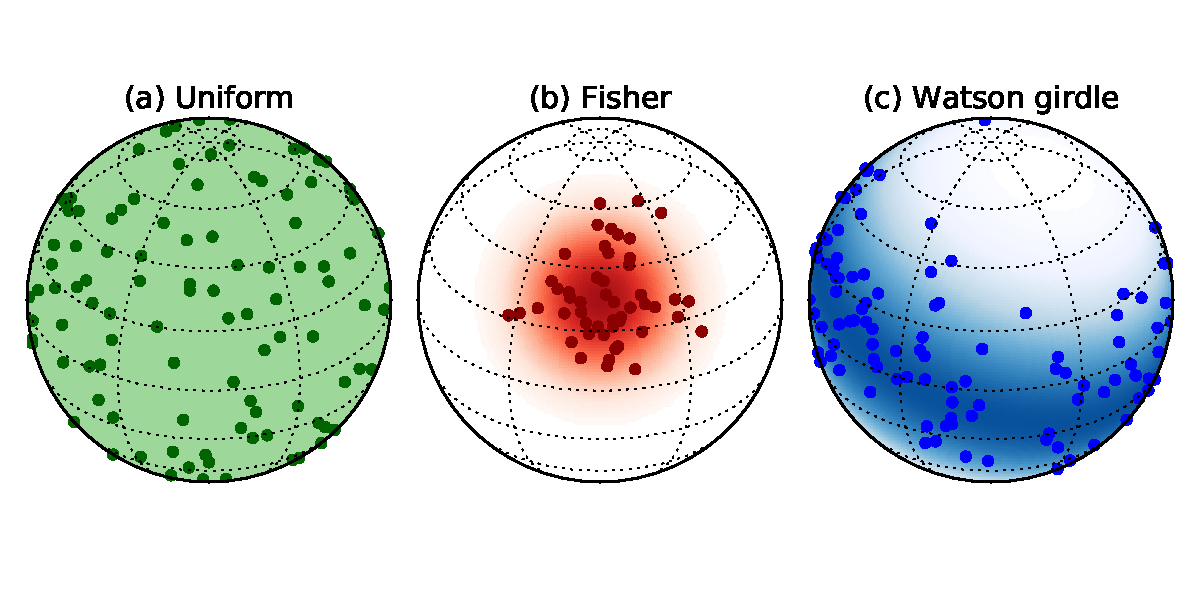
\includegraphics[width=0.9\textwidth]{figures/cartoon/distributions.pdf}
\caption[Spherical probability distributions.]{Probability densities for distributions of directional data, as well as samples drawn from them. All are plotted using an orthographic projection. (a) Uniform distribution. (b) Fisher distribution. The center of the distribution is at $30^\circ$N, $30^\circ$E, and the concentration parameter $\kappa=20$. (c) Watson girdle distribution. The pole of symmetry is at $70^\circ$N, $90^\circ$E, and the concentration parameter $\kappa=-5$.}
\label{fig:distributions}
\end{figure*}

The simplest probability distribution on a sphere is the spherical uniform distribution.
It has a probability density given by
\begin{equation}
  \rho_U(\phi, \psi) = \frac{1}{4 \pi},
\end{equation}
where $\rho_U$ is the probability density, $\phi$ is the longitude, and $\psi$ is the latitude
(we will also refer to the Cartesian unit vector $\hat{\mathbf{x}}$ as a concise representation of $\phi$ and $\psi$).
Most non-uniform distributions on a sphere reduce to the uniform distribution in some limit.
We will use this distribution when we want to specify an uninformative prior for directional parameters.

\subsubsection{Fisher distribution}
The Fisher distribution (also called the von Mises-Fisher distribution) is the analogue
of a 2D normal distribution on a sphere.
The probability density $\rho_F$ at a point $\hat{\mathbf{x}}$ is given by
\begin{equation}
  \begin{aligned}
  \rho_F(\phi, \psi ; \kappa_F, \hat{\mitbf{\mu}}) 
  &= \frac{1}{C_F} \exp \left( \kappa_F \hat{\mathbf{x}}^T \hat{\mitbf{\mu}} \right) \\
  &= \frac{1}{C_F} \exp \left( \kappa_F \cos \theta \right),
  \end{aligned}
\end{equation}
where $\kappa_F$ is the concentration of the distribution, 
$\hat{\mitbf{\mu}}$ the unit vector for the mean direction of the distribution, 
and $C_F$ is a normalization coefficient. It can be alternatively
parameterized using $\theta$, which is the angle between $\hat{\mathbf{x}}$ and $\hat{\mitbf{\mu}}$.
The normalization factor is given by 
\begin{equation}
  C_F = \frac{\kappa_F}{4 \pi \sinh{\kappa_F}}.
\end{equation}
When $\kappa_F$ goes to zero, the Fisher distribution is equivalent to the spherical uniform distribution.

The position and uncertainty of most paleomagnetic poles are represented by Fisher distributions,
and so we will use it to calculate the likelihood function for pole directions in the model.

\subsubsection{Watson girdle distribution}
Whereas the Fisher distribution concentrates probability density near around a pole on
the surface of the sphere, the Watson girdle probability distribution is concentrated
in a belt orthogonal to the pole. It is useful for characterizing planar data, and is given by
\begin{equation}
  \begin{aligned}
  \rho_W(\phi, \psi; \kappa_W, \hat{\mitbf{\mu}}) 
  &= \frac{1}{C_W} \exp \left( \kappa_W (\hat{\mathbf{x}}^T \hat{\mitbf{\mu}})^2 \right) \\
  &= \frac{1}{C_W} \exp \left( \kappa_W \cos^2 \theta \right),
  \end{aligned}
\label{eq:watson}
\end{equation}
where $\kappa_W$ is the concentration of the girdle, $C_W$ is a normalization coefficient,
and the other parameters are identical to those in the Fisher distribution.
The Watson distribution is girdle-shaped only when $\kappa_W$ is a negative number, 
which is the only case we consider here.
The normalization factor is given by
\begin{equation}
  C_W = \left[ {}_1 F_1 \left( \frac{1}{2}, \frac{3}{2}, \kappa_W \right) \right]^{-1},
\end{equation}
where ${}_1 F_1()$ is Kummer's confluent hypergeometric function, which is available
in most software libraries of special mathematical functions.
As with the Fisher distribution, when $\kappa_W$ goes to zero, 
the Watson distribution is equivalent to the spherical uniform distribution.

\section{A model for PEP inversion}
\label{sec:model}
\subsection{Forward model}
\label{sec:forward_model}
The forward model for PEP analysis in this study is essentially unchanged from that of \citet{gordon1984paleomagnetic}.
We describe plate motions (and hence paleomagnetic pole motions) with a series of Euler poles.
Each Euler pole has three parameters for which we are inverting (a latitude, a longitude, and a rotation rate).

We furthermore need to specify the ages where we transition from 
one Euler pole to the next (the cusps, or ``hairpins'' of \citet{irving1972hairpins}).
In the context of parameter inversion these are often known as ``changepoints.''

Finally, we need a starting position on the globe, which, in practice, can be sampled
from the Fisher distribution of the oldest paleomagnetic pole in the dataset.
The starting point contributes two parameters (a latitude and a longitude).

All together, this means that an inversion for $n_e$ Euler poles will
have $3 n_e$ parameters for the poles, $(n_e-1)$ parameters for the changepoints,
and 2 parameters for the starting location.
The number parameters for which we are inverting is then given by
\begin{equation}
\begin{aligned}
N &= 3 n_e + (n_e -1) + 2 \\
 &= 4 n_e + 1.
\end{aligned}
\label{eq:n_parameters}
\end{equation}

For each Euler pole $\mitbf{\omega}_i$ the velocity $\mathbf{v}$ of a point 
$\mathbf{p}$ on the surface of the globe is given by
\begin{equation}
\mathbf{v} = \mitbf{\omega}_i \times \mathbf{p}.
\label{eq:rigid_rotation}
\end{equation}
Finite rotations can be performed by constructing Euler angle rotation matrices \citep[cf.][]{goldstein1965classical}. 
We generate synthetic paleomagnetic pole positions from the forward model by stringing together
finite rotations through the stage poles until the age of the paleomagnetic pole
is reached. These positions can then be compared to the actual paleomagnetic poles in our dataset.

\subsection{Choice of prior distributions}
\label{sec:priors}

Bayesian analysis requires us to specify prior probability distributions 
for each of the model parameters in the inverse problem.
These distributions reflect our state of belief about the values of the parameters before we begin,
and allow us the option of incorporating information otherwise not captured by the model.
To avoid biasing the results of the model towards a specific posterior distribution,
we usually try to choose as prior distributions to be as uninformative as possible. 
Depending upon the context, and the type of parameter, that choice may vary.
The central parameters in the paleomagnetic Euler pole problem are the Euler pole positions,
the Euler pole magnitudes, the changepoints, the starting point, and the paleomagnetic pole ages, which we treat in turn.
We use the notation $x \sim y$ to indicate that the parameter $x$ is drawn from distribution $y$.

\textbf{Euler pole directions:} 
The first parameter we consider is the position of the Euler poles, which should be drawn
from a spherical probability distribution.
The least informative prior distribution for the i'th Euler pole is the uniform spherical distribution:
\begin{equation}
\hat{\mitbf{\omega}}_i \sim \rho_U.
\end{equation}
essentially allowing the Euler pole to be anywhere on the globe with equal probability.

An interesting alternative choice is to inform our prior distribution for Euler pole position based
on current plate motions. It has long been observed that, to first order, plate motions
are well explained by slab-pull torques acting along subduction zones, and to a lesser
extent, ridge push and continental keel effects \citep{forsyth1975relative, gordon1978absolute, richardson1992ridge}.
This observation is explained by the fact that plate tectonics is the 
surface expression of Earth's convection.

We can then ask the question of whether the Euler pole for a given plate is more likely
to be on top of the plate (corresponding to a spinning motion for that plate) or far away
from that plate (corresponding to motion across the surface of Earth).
Given the convective interpretation of plates, we can hypothesize that the second possibility
is more likely because a spinning plate has no divergence 
(i.e., spreading centers and subduction zones, \citep{forte1987plate, gable1991convection}). 
Without spreading centers or subduction zones the plate motion does not contribute to convection.

To test this hypothesis, we generated position samples on the surface of Earth and computed
the angular distance between that point and the Euler pole for the plate in which that point resides.
We used the NNR-MORVEL56 model for current plate motions \cite{argus2011geologically}
and restricted our analysis to the fourteen largest plates.
We then fit those angular distance samples to a Watson girdle distribution (Equation~\eqref{eq:watson}), 
inverting for the concentration parameter $\kappa_W$.
We find that the distribution is best fit with $\kappa_W \approx -0.8$, which corresponds
to the Euler pole probability density being roughly twice as large $90^\circ$
away from a given point than on top of the point (see Figure~\ref{fig:euler_pole_prior}.

\textbf{Euler pole magnitudes:} 
The magnitude of each Euler pole is a strictly positive number, specifying the
rotation rate of that pole (negative rotations can be accommodated by flipping an Euler
pole to the antipode).
There are several possibilities for the prior distribution for the rates.
In order to not bias the inversion towards a particular
rate we can choose a uniform prior distribution with large support:
\begin{equation}
\vert \mitbf{\omega}_i \vert \sim U(0, 4),
\end{equation}
where $U(\cdot, \cdot)$ is a uniform distribution between two values, and is specified 
in degrees per Myr. Typical rotation rates for present day plate motions
are under $1^\circ$/Myr \citep{argus2011geologically}, which corresponds to rates
of about 13 cm/yr at a position $90^\circ$ from the pole.

Another option is to choose a weakly informative prior distribution for the Euler pole magnitudes
informed by recent plate motions (similar to the Watson girdle prior distribution for the directions).
\citet{zahirovic2015tectonic} found based on Cenozoic and Mesozoic plate reconstructions
that plate speeds much higher than 15 cm/yr were unlikely.
A reasonable choice of distribution for strictly positive numbers is the exponential distribution,
given by
\begin{equation}
\rho_E(\vert \mitbf{\omega}_i \vert) = \lambda \exp(-\lambda \vert \mitbf{\omega}_i \vert),
\end{equation}
which has higher probability density at lower values, and falls off exponentially.
We sampled the current plate rates on Earth's surface according to NNR-MORVEL56
and fit those to an exponential distribution. The best fitting scale parameter $\lambda$
for current plate rates is $\lambda\approx2.5$.
Making this choice of prior distribution for Euler pole rotation rates can be seen as a form
of regularization on plate speeds.

\begin{figure*}
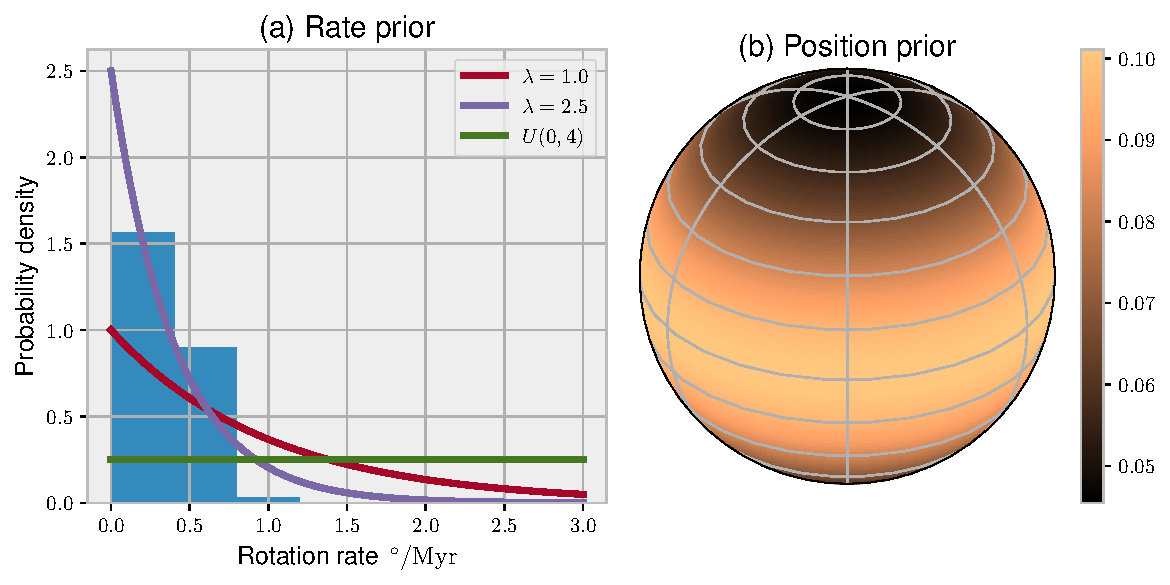
\includegraphics[width=0.9\textwidth]{figures/euler_pole_prior/euler_pole_prior.pdf}
\caption[Informative prior distributions for Euler poles]{Informative prior distributions for Euler poles. (a) Prior probabilities for rotation rates. The histogram is the angular rotation rate from one thousand samples from the surface of Earth, using the NNR-MORVEL56 model. A fit to this sample set with an exponential distribution yields a scale parameter of $\lambda \approx 2.5$. We also show the distribution for $\lambda = 1.0$, which imposes less regularization on the rate. (b) Prior probability density for the position of the Euler poles. We again sampled one thousand points on Earth's surface, calculating the angular distance between that point and the Euler pole for its plate. Fitting the resulting angular distribution to a Watson girdle distribution finds $\kappa_W \approx -0.8$. This results in a probability density roughly twice as large at the equator as at the pole.}
\label{fig:euler_pole_prior}
\end{figure*}

\textbf{Changepoints:} 
Changepoints occur sequentially between the oldest (at age $a_\mathrm{max}$) and
youngest (at age $a_\mathrm{min}$) paleomagnetic poles.
We choose a uniform distribution as a prior for these changepoints:
\begin{equation}
c_i \sim U( a_\mathrm{min}, a_\mathrm{max}),
\end{equation}
where $c_i$ is the i'th changepoint.

\textbf{Starting position:}
Finally, the starting position $\hat{\mathbf{x}}_\mathrm{start}$ for the set of Euler pole rotations needs a prior distribution.
We could choose another uniform distribution, but a more reasonable choice
is to start from near the oldest paleomagnetic pole in the dataset.
We therefore choose the Fisher distribution of the oldest paleomagnetic pole as a reasonable prior distribution for a start point:
\begin{equation}
\hat{\mathbf{x}}_\mathrm{start} \sim \rho_F(\kappa_{F0}, \hat{\mitbf{\mu_0}}),
\end{equation}
where $\kappa_{F0}$ and $\hat{\mitbf{\mu}}_0$ are the concentration parameter and mean direction
of the oldest paleomagnetic pole in the dataset.

\textbf{Pole ages:}
One of the major advantages of Bayesian analysis is the ability to naturally incorporate
uncertainties in as many parameters as we need. Previous approaches to
modeling APW paths have the drawback that they do not easily account for uncertainties in
the age of paleomagnetic poles. In our approach we can include age uncertainty
by including the age of the poles and associated uncertainty as parameters in our model.

There are many different ways to constrain the ages of the geologic units from
which we obtain paleomagnetic poles, including radiometric dating, biostratigraphy,
magnetostratigraphy, cross-cutting relationships, and stratigraphic relations.
Here we concentrate on poles that are either interpreted to be the age of a single radiometric
date or are interpreted to be bracketed stratigraphically between two dates
(derived radiometrically or by using other age control such as biostratigraphy).
If a geologic unit has been radiometrically dated, we can model the age of
the j'th paleomagnetic pole $a_j$ as a normal distribution with mean $\mu_j$ and standard deviation $\sigma_j$:
\begin{equation}
a_j \sim N(\mu_j, \sigma_j),
\end{equation}
where $N(.,.)$ denotes a normal distribution.

Freqently, however, the geologic unit from which we obtain a paleomagnetic pole
is not well dated, but its age can be constrained to lie between those
of well-dated units stratigraphically above and below it. In this case,
we argue that a uniform distribution between those ages is a reasonable choice
of prior distribution:
\begin{equation}
a_j \sim U(a_\mathrm{young}, a_\mathrm{old}),
\end{equation}
where $a_\mathrm{young}$ and $a_\mathrm{old}$ are the ages of the lower and upper
age constraints, respectively.

To summarize our choices for prior distributions:
\begin{itemize}
\item Euler pole positions: spherical uniform distribution, or a Watson girdle distribution with $\kappa_W \approx -0.8$.
\item Euler pole magnitudes: Uniform distribution between 0$^\circ$ and 4$^\circ$/Myr, or an exponential distribution with $\lambda \approx 2.5$.
\item Changepoints: uniform distribution between $a_\mathrm{min}$ and $a_\mathrm{max}$.
\item Paleomagnetic pole ages: normal or uniform distribution, depending on the type of age control for the geologic unit.
\end{itemize}


\subsection{Likelihood}
\label{sec:likelihood}
In addition to the choice of prior distributions we need a statistical description of the observations.
This description will allow us to calculate the likelihood function, which, when combined with the prior distributions,
allows us to evaluate Bayes' theorem (Equation~\eqref{eq:propbayes}).

In the case of APW paths, our observations are paleomagnetic poles.
The most common statistical distribution for describing paleomagnetic poles is the Fisher distribution
(though others are possible, such as the Kent or Bingham distribitions, c.f. \citet{tauxe2009essentials}).
Given the set of model parameters $\mathbf{m}$ and the forward model $\mathbf{g}(\mathbf{m})$, described
in Section~\ref{sec:forward_model}, we can calculate the predicted paleomagnetic pole unit vectors $\hat{\mathbf{x}}_{p,i}$.
For a set of $n$ paleomagnetic poles, the likelihood is then given by the product of the probabilities
of each observation:
\begin{equation}
P(\mathbf{d} \vert \mathbf{m}) = \displaystyle\prod_{i=1}^n \frac{1}{C_{F,i}} \exp \left( \kappa_{F,i} \hat{\mathbf{x}}_{p,i}^T \hat{\mitbf{\mu}}_i \right).
\label{eq:model_likelihood}
\end{equation}

\section{Example inversions}
\label{sec:example_inversion}

Before proceeding with inversions for paleomagnetic Euler poles using real paleomagnetic data,
it is useful to consider a few examples of inversions for synthetic datasets.
We have implemented the forward model described in Section~\ref{sec:forward_model}
in Python, and used the package PyMC \citep{patil2010pymc} to perform the Monte Carlo inversion.
We use a Metropolis-Hastings sampler, starting from a fit to the maximum a posteriori (MAP) probability.
In most cases shown here we generate $10^6$ samples, discarding the first 20\% to avoid
potential bias in the posterior due to a poor starting point.

In all of the inversions we show here, we choose $\kappa_W=0$ for the Watson concentration parameter
in the Euler pole direction prior distribution (that is, equivalent to a uniform distribution on a sphere),
and $\lambda=2.5$ for the scale parameter in the Euler pole magnitude prior distribution.

\subsection{One stage pole}
\label{sec:one_stage_pole}
We begin by trying to recover the Euler pole for a single rotation.
We generate a synthetic APW track of four poles by starting from a pole at $0^\circ$ N, $30^\circ$ E,
and rotating around an Euler pole at $0^\circ$ N, $0^\circ$ E for 180 Myr at a rate of $1^\circ$/Myr.
We produce paleomagnetics pole at 190 Ma, 130 Ma, 70 Ma, and 10 Ma, and prescribe A95
of $10^\circ$ to each pole (where A95 indicates the 95\% angular confidence interval for the pole position).

The results of the inversion are shown in Figure~\ref{fig:one_euler_pole}.
The Bayesian approach successfully recovers a posterior probability distribution for the position
of the Euler pole that includes the start pole, as well as a rate that is centered
near the true value of $1^\circ$/Myr. The posterior distribution for the rate
has a highest posterior density (HPD) credible interval at 95\% 
(which we abbreviate from here as a 95\% credible interval)
between $0.8^\circ$/Myr and $1.2^\circ$/Myr, reflecting the resolving power of the inversion.

\begin{figure*}
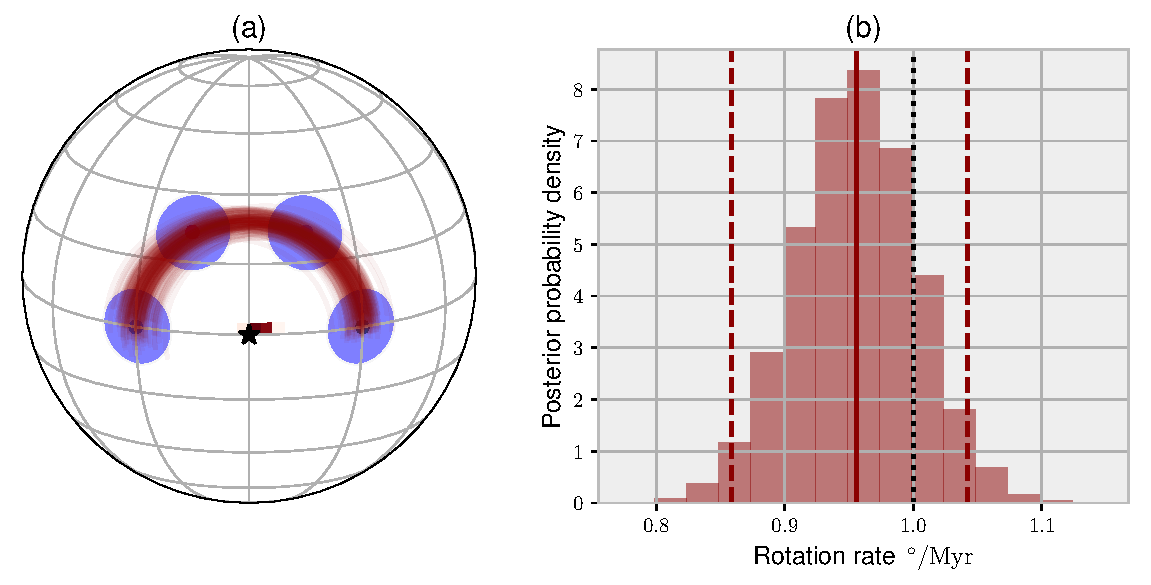
\includegraphics[width=0.9\textwidth]{figures/synthetic/one_euler_pole.pdf}
\caption[Inversion for a single paleomagnetic Euler pole.]{Inversion for a single paleomagnetic Euler pole. (a) Four paleomagnetic poles are generated during a net $180^\circ$ rotation about an Euler pole at $0^\circ$N, $0^\circ$E over 180 Myr, for a rotation rate of $1^\circ$/Myr. The red distribution is the probability density function recovered by MCMC inversion, and the red lines are a sampling of 200 synthetic APW paths generated by the inversion. (b) Posterior probability density for the rotation rate of the Euler pole recovered by the inversion. The solid line shows the median of the distribution ($1^\circ$/Myr), and the dashed lines show the 95\% credible interval ($0.8^\circ-1.2^\circ$/Myr). }
\label{fig:one_euler_pole}
\end{figure*}

\subsection{Two stage poles}
\label{sec:two_stage_poles}
We next consider an inversion for an APW path with two stage poles.
Unlike the example in Section~\ref{sec:one_stage_pole}, this inversion also requires a changepoint.
We generate five paleomagnetic poles from a starting point at $0^\circ$ N, $60^\circ$ W.
The first rotation is around an Euler pole at $41^\circ$ N, $60^\circ$ W, and rotates at $1^\circ$/Myr for 130 Myr.
The rotation rotation is around an Euler pole at $41^\circ$ N, $60^\circ$ E, rotates at the same rate for the same amount of time.
The ``observations'' produced by the two stage model are shown in Figure~\ref{fig:two_euler_poles}.
The inversion successfully recovers the Euler pole positions and rates, and the changepoint is centered near 130 Ma.
\begin{figure*}
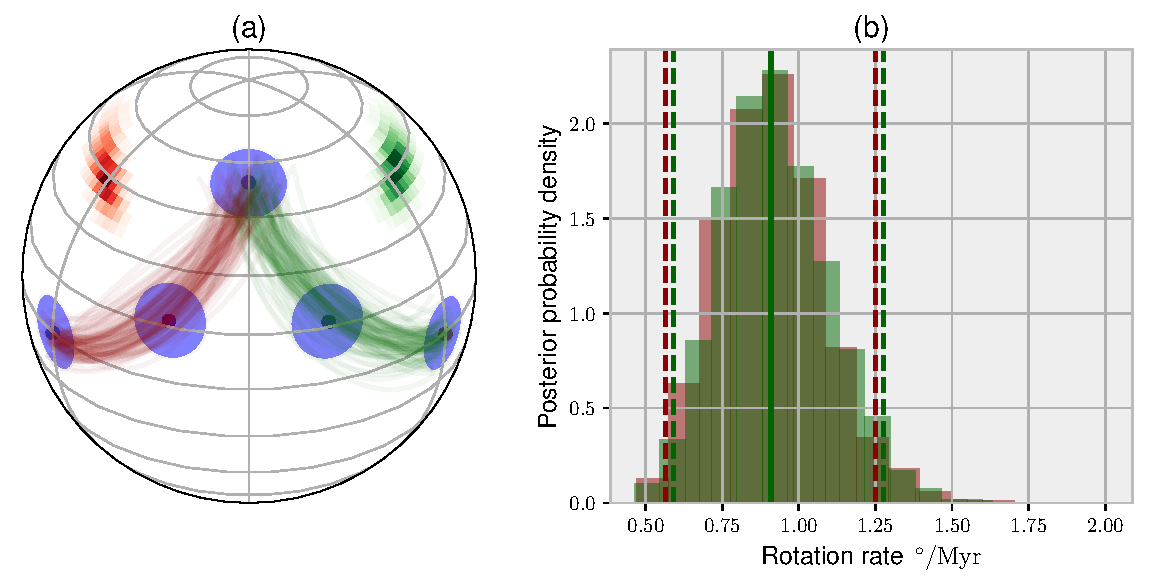
\includegraphics[width=0.9\textwidth]{figures/synthetic/two_euler_poles.pdf}
\caption[Inversion for two successive paleomagnetic Euler poles.]{Inversion for two successive paleomagnetic Euler poles. (a) Five paleomagnetic poles are generated, beginning with a pole at $0^\circ$N, $60^\circ$W. The first Euler pole is located at $41^\circ$N, $60^\circ$W, and rotates at $1^\circ$/Myr for 130 Myr. The second Euler pole is located at $41^\circ$N, $60^\circ$E, and rotates at the same speed and for the same duration. The red and green distributions show the location of the first and second Euler poles (respectively) recovered by the MCMC inversion. The the red and green lines are a sampling of 200 synthetic APW paths generated by the inversion. (b) Posterior probability density for the rotation rates of the Euler poles recovered by the inversion. The solid lines show the median values of the distributions ($\sim 0.97^\circ$/Myr, and the dashed lines show the 95\% credible intervals ($\sim 0.61^\circ-1.3^\circ$/Myr). The two distributions are nearly identical, and centered on the true value of the rate.}
\label{fig:two_euler_poles}
\end{figure*}


\subsection{Incorporating age uncertainty}
\label{sec:age_uncertainty}
A major benefit of the Bayesian approach to inverse problems is its great generality.
As long as some effect can be described statistically and incorporated into our
forward model, we can include it in the inverse problem.

In this case, we include uncertainties in the ages of the paleomagnetic poles.
We use the same test case as in Section~\ref{sec:one_stage_pole}, but assign uncertain prior
distributions to the ages of the poles. For the first and last poles we assume they
are radiometrically dated with standard deviations of 2 Myr.
However, we assume that the middle two poles have no age control, except that their
respective rock units lie stratigraphically between the first and last poles.
We thus assign Gaussian prior distributions to the first and last poles and uniform prior distributions
to the middle two.

The primary effect of adding uncertainties to the ages of the poles is that they can
help to constrain the location of the APW path without providing an unwanted constraint
on the timing of the path.
Figure~\ref{fig:age_uncertainty_samples} shows the prior and posterior distributions for the
ages of the poles. We can see from the posterior distribution that the inversion
successfully places the ages of the middle two poles at $\sim70$ Ma and $\sim130$ Ma,
though with relatively wide 95\% credible intervals.
The posterior distributions for the Euler pole position and magnitude 
which we recover from this inversion are visually identical to those in Figure~\ref{fig:one_euler_pole}.

\begin{figure*}
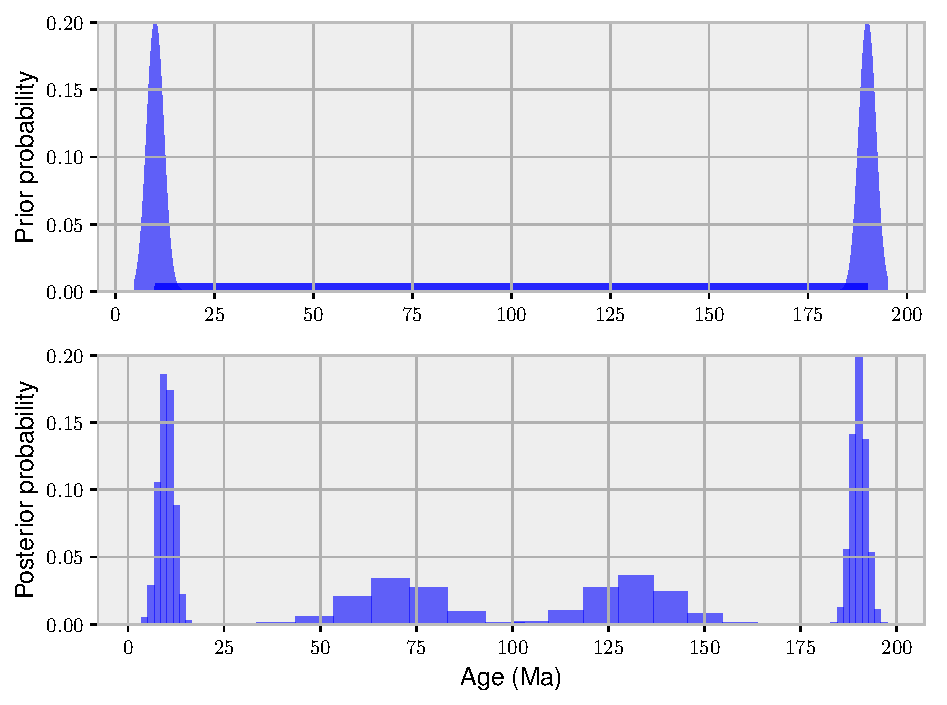
\includegraphics[width=0.9\textwidth]{figures/synthetic/age_uncertainty_samples.pdf}
\caption[Probability distributions for ages of the paleomagnetic poles in the one-Euler pole inversion test.]{Probability distributions for the ages of the paleomagentic poles in the one-Euler pole inversion test. Top: prior distributions. We presume the first and last poles to be radiometrically dated with one-sigma uncertainties of 2 Myr, and are assigned Gaussian prior distributions. The middle two poles are undated, and are only stratigraphically constrained to be between the first and last poles. Bottom: posterior distributions after $10^5$ MCMC samples. The distributons of the first and last samples are largely unchanged, but the distributions for the middle two poles are centered on their true values of 70 Ma and 130 Ma. Importantly, the middle poles help to constrain the location of the Euler pole, but the wide prior distributions on their ages do little to constrain the rotation rates.}
\label{fig:age_uncertainty_samples}
\end{figure*}

\section{Application to Cenozoic Australian APW path}
\label{sec:australia}
%%\clearpage
A first application of our model for PEP inversion is with the case of Cenozoic Australia.
Australia's Cenozoic plate motions are relatively well constrained by oceanic fracture zones
and hotspot volcanism \citep{muller1993revised, seton2012global}.
This gives us the opportunity to compare the results of our model to those known motions.

\begin{table}
\scriptsize
\begin{tabular}{p{4cm} p{1.0cm} p{1.0cm} p{1.0cm} p{2.5cm} p{1cm} p{1cm}}
\toprule
                                         Pole &  $\psi_p$ &  $\phi_p$ &  $A_{95}$ &               Reference &  Lower age (Ma) &  Upper age (Ma) \\
\midrule
           Werriko Limestone, Newer Volcanics &      83.2 &     283.6 &       6.2 &  \cite{idnurm1985lateI} &               1 &               5 \\
 Port Campbell Limestone, Glenample Formation &      77.2 &     303.5 &       4.2 &  \cite{idnurm1985lateI} &               6 &              20 \\
                        Point Addis Limestone &      68.4 &     298.7 &       4.8 &  \cite{idnurm1985lateI} &              23 &              29 \\
                       Browns Creek Formation &      65.5 &     292.5 &       2.5 &    \cite{idnurm1994new} &              35 &              40 \\
                     North Rankin 1 Drillcore &      61.7 &     298.4 &       5.1 &  \cite{idnurm1985lateI} &              56 &              62 \\
\bottomrule
\end{tabular}

\caption[Paleomagnetic poles used for the Australia inversion.]{Paleomagnetic poles used for the Australia inversion, as well as references. 
$\psi_p$ and $\phi_p$ give the latitude and longitude of the mean pole position, and A95 gives the 95\% angular confidence interval for that position.
The paleomagnetic poles come primarily from sedimentary successions with biostratigraphic age control 
(with the exception of the Newer Volcanics, which erupted from $\sim2-4$ Ma).
Upper and lower age bounds come from estimates from \citet{idnurm1985lateI} and version 4.6 of the Global paleomagnetic databad (GPMDB). }
\label{tab:australia_poles}
\end{table}

The most reliable Cenozoic Australian paleomagnetic data comes from \citet{idnurm1985lateI} and \citet{idnurm1994new}.
Earlier paleomagnetic poles exist, but they show considerably more scatter,
and there are concerns that they do not adequately average secular variations
\citep{idnurm1985lateI, klootwijk2009sedimentary}.
\citet{idnurm1985lateII} found that the latitude-age progression of the paleomagnetic
data was significantly faster than that given by hotspot tracks.
He proposed that the best explanation for this discrepancy was a long-lived
departure of Earth's magnetic field from a geocentric axial dipole (GAD).

Here we reanalyze the available paleomagnetic data with our statistical model,
which allows us to incorporate more recnet models for Australia's plate motions
and perform an accounting of the uncertainties within our Bayesian framework.
The pole list we use is given in Table~\ref{tab:australia_poles}.
We fit the paleomagnetic pole list to one and two PEPs, and compared them
to the global plate motion model from \citet{seton2012global}.

Figure~\ref{fig:australia_paths_1} shows the results for a single Euler pole
plotted on the globe, as well as modeled paleomagnetic poles drawn from the posterior distribtuion. 
Figure~\ref{fig:australia_speeds_1}b shows the single Euler pole result plotted as latitude vs. age.
Both the paleomagnetic data and the \citet{seton2012global} model show a speed-up in
Australia's motion as it approaches the present day, though the paleomagnetic data
has systematically higher recent latitudes, implying faster plate speeds.
While the single Euler pole fit does a reasonable job of fitting the azimuth of the plate motion model 
(Figure~\ref{fig:australia_paths_1}), it has difficulty fitting that change in speed, 
and does not pass through all the paleomagnetic poles in Figure~\ref{fig:australia_speeds_1}b.

\begin{figure*}
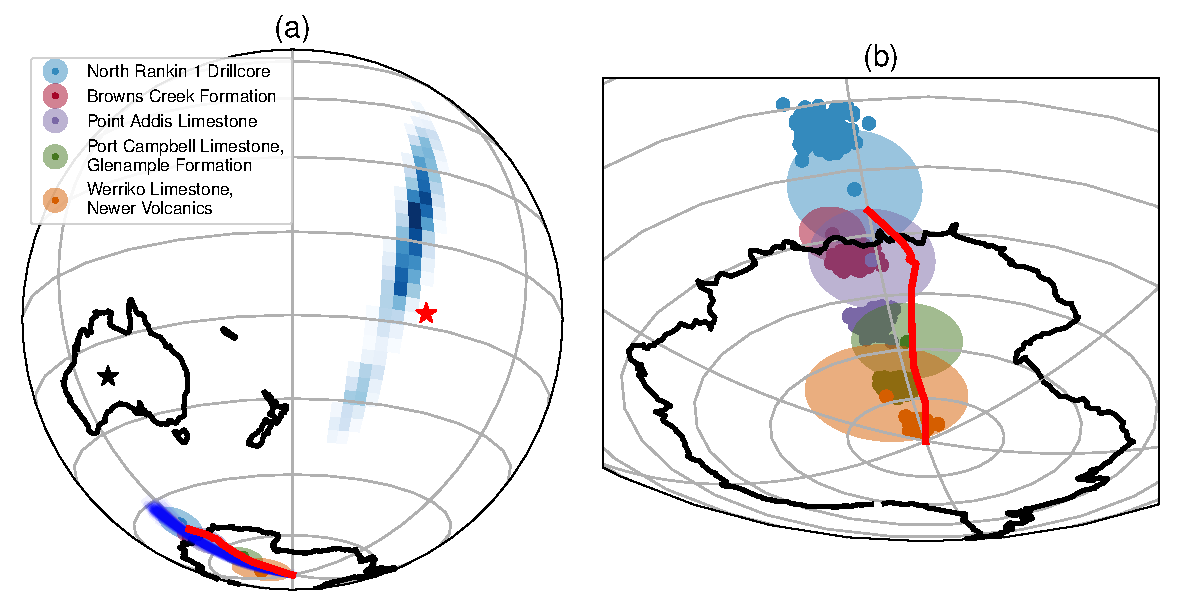
\includegraphics[width=0.9\textwidth]{figures/australia/australia_paths_1.pdf}
\caption[Australian Cenozoic APW path fit to one Euler rotation.]{Australian Cenozoic APW path fit to one Euler rotation. 
(a) Euler pole position and sample tracks. The blue distribution shows the posterior distribution of Euler pole positions, and the blue paths show a sampling of paths drawn from the posterior. The red line shows the polar wander path derived from the global plate motion model of \citet{seton2012global}, and the red star shows the average Euler pole from 0-60 Ma defined by the \citet{seton2012global} path. We calculate plate speeds referenced to Uluru, shown by the black star.
(b) Paleomagnetic pole positions for draws from the posterior distribtion of the inversion superimposed on observed pole positions and their uncertainty.}
\label{fig:australia_paths_1}
\end{figure*}

\begin{figure*}
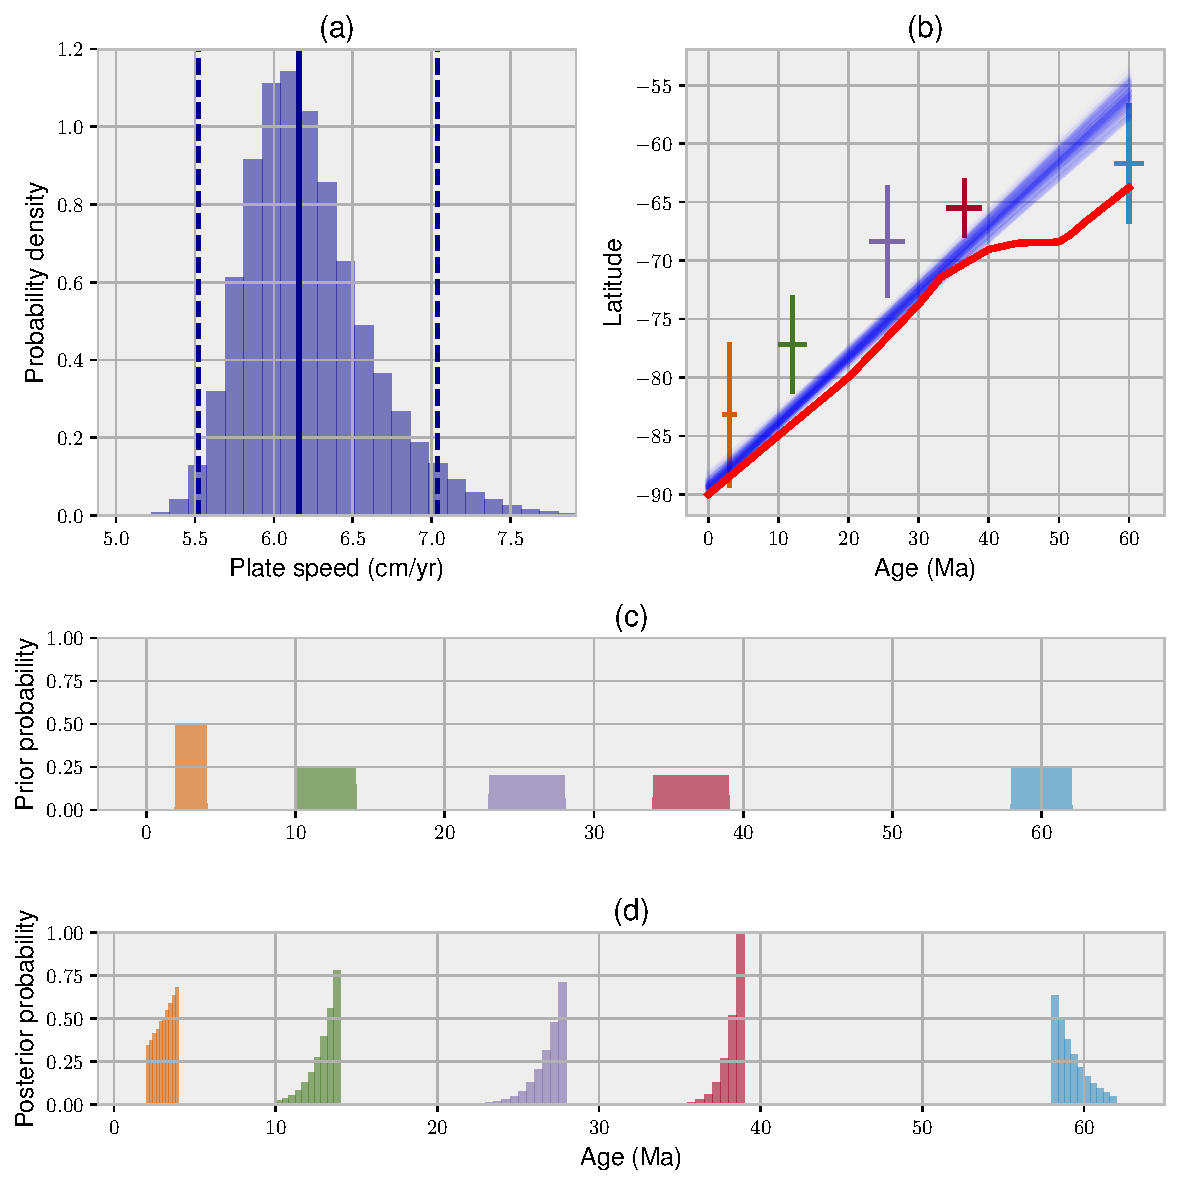
\includegraphics[width=0.9\textwidth]{figures/australia/australia_speeds_1.pdf}
\caption[Results for Australian Cenozoic APW path with one Euler rotation.]{Results for Australian Cenozoic APW path with one Euler rotation. 
(a) Posterior distribution for plate speed. The solid line shows the median plate speed (6.2 cm/yr) and the dashed lines show the 95\% credible interval (5.4-8.1 cm/yr).
(b) Latitude vs. age. The paleomagnetic poles are shown as data points, with age and latitude uncertainty. The blue lines show a sampling of the posterior path distribution, and the red line shows the \citet{seton2012global} plate motion model. Note that the paleomagnetic poles are systematically above the \citet{seton2012global} model, and that the single Euler rotation path is not able to pass through all the data points.
(c) Prior distributions for the ages of paleomagnetic poles.
(d) Posterior distributions for the ages of paleomagnetic poles.}
\label{fig:australia_speeds_1}
\end{figure*}

The two-Euler pole inversion, shown in Figures~\ref{fig:australia_paths_2}-\ref{fig:australia_speeds_2} does a better job of
fitting the paleomagnetic poles, preferring a change in speed at $\sim 23$ Ma.
However, the $\sim23-0$ Ma speeds are significantly faster than those from the global plate motion model,
consistent with the conclusions of \citet{idnurm1985lateII}.
We conclude that the discrepancy between the Australian paleomagnetic data and
Cenozoic plate motion models remains.

\begin{figure*}
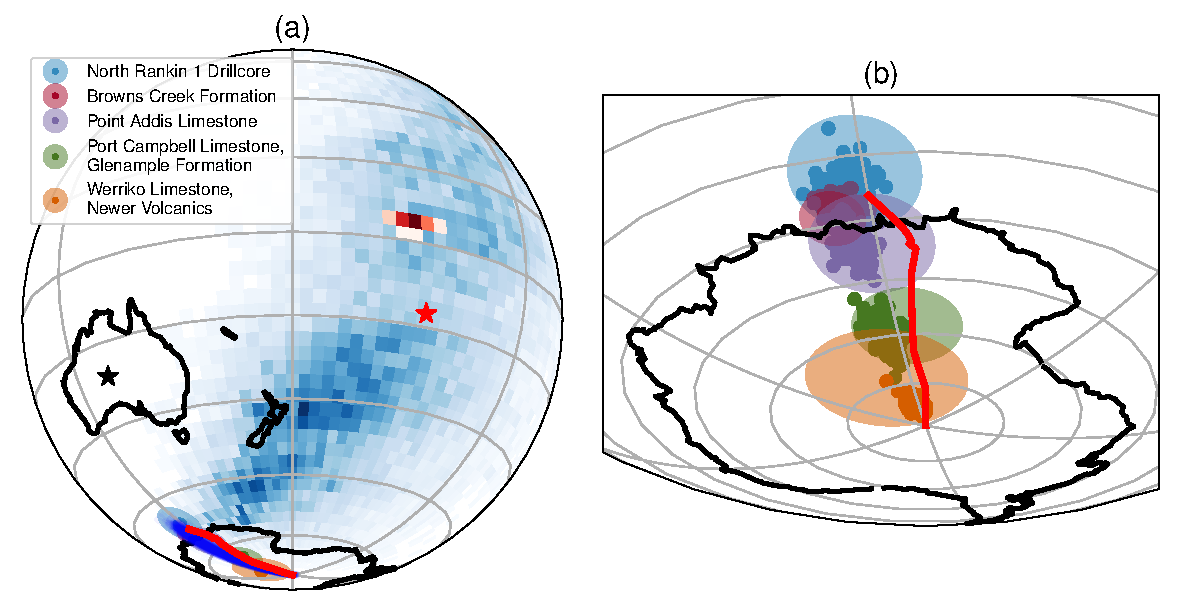
\includegraphics[width=0.9\textwidth]{figures/australia/australia_paths_2.pdf}
\caption[Australian Cenozoic APW path fit to two Euler rotations.]{Australian Cenozoic APW path fit to two Euler rotations. 
(a) Euler pole locations and sample tracks. The blue distribution shows the posterior of positions for the first Euler pole, and the red distribution shows the posterior for the second Euler pole. The distribution of the first Euler pole is quite broad, reflecting the short length of the portion of the path that it is trying to fit (shorter paths provide less of a constraint on the position). The the blue paths show a sampling of paths drawn from the posterior. As in Figure~\ref{fig:australia_paths_1}, the red line shows the polar wander path derived from the global plate motion model of \citet{seton2012global}, and the red star shows the average Euler pole from 0-60 Ma defined by the \citet{seton2012global} path.
(b) Paleomagnetic pole positions for draws from the posterior distribtion of the inversion superimposed on observed pole positions and their uncertainty.}
\label{fig:australia_paths_2}
\end{figure*}

\begin{figure*}
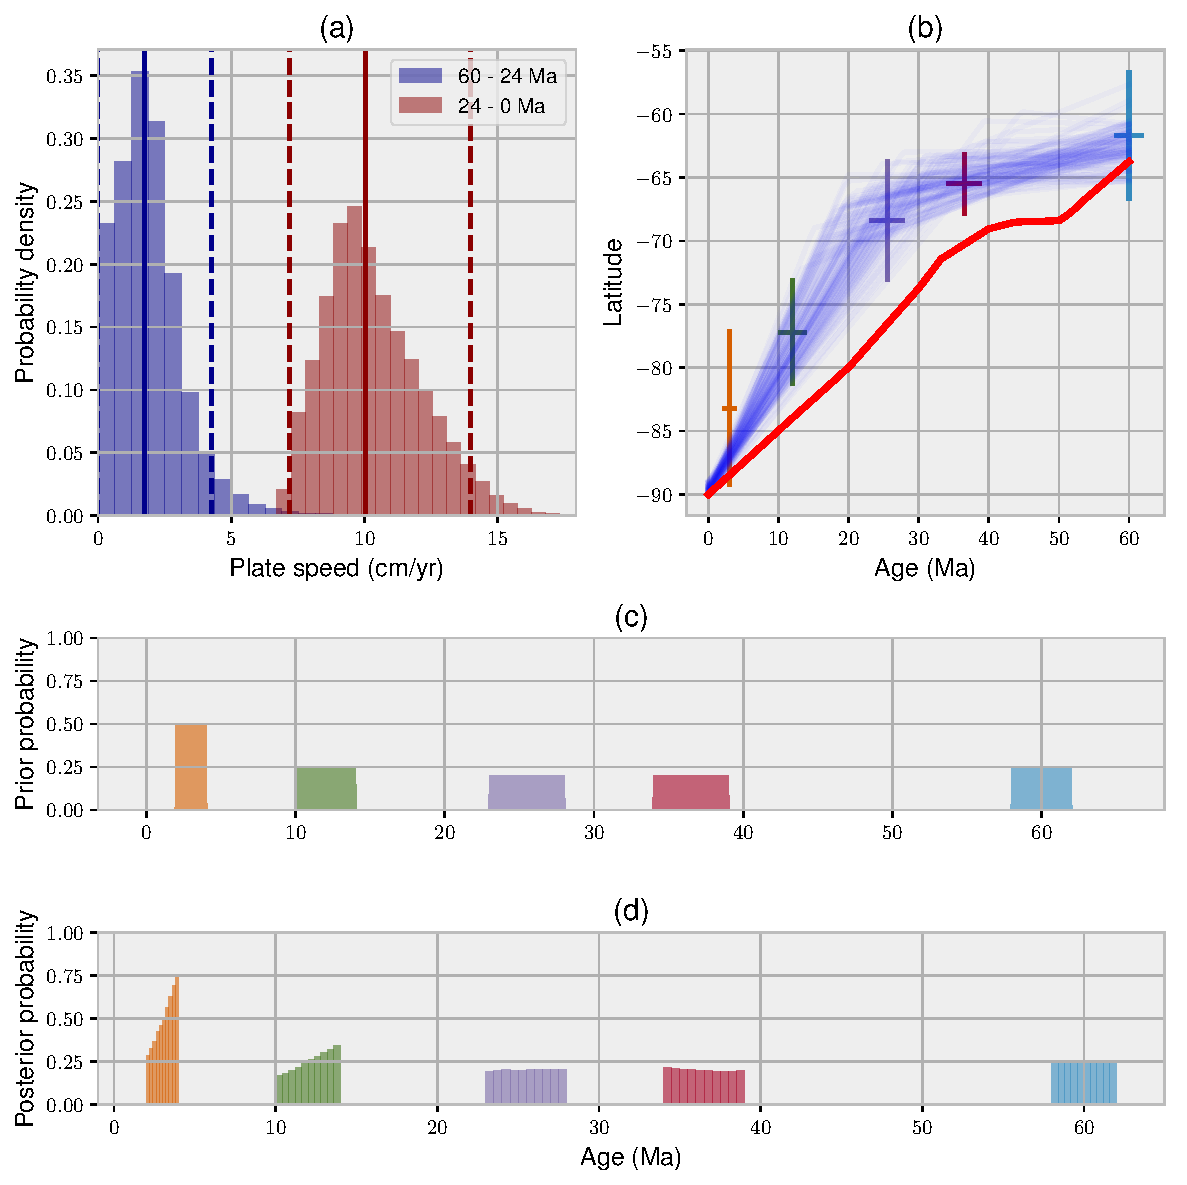
\includegraphics[width=0.9\textwidth]{figures/australia/australia_speeds_2.pdf}
\caption[Results for Australian Cenozoic APW path with two Euler rotations.]{Results for Australian Cenozoic APW path with two Euler rotations. 
(a) Posterior distributions for plate speeds. The blue distribution shows the plate speeds for the first rotation, which occurs from approximately 60-23 Ma. The red distribution shows the plate speeds for the second rotation, which occurs from approximately 23-0 Ma. The changepoint is approximate, since it is also a random variable with its own posterior distribution. This inversion prefers a slow first rotation (2.2 cm/yr with a 95\% credible interval of 0-7.3 cm/yr) and a fast second rotation (11.8 cm/yr with a 95\% credible interval of 7.1-19 cm/yr).
(b) Latitude vs. age. The paleomagnetic poles are shown as data points, with age and latitude uncertainty. The blue lines show a sampling of the posterior path distribution, and the red line shows the \citet{seton2012global} plate motion model. Compared to the single Euler pole fits (Figure~\ref{fig:australia_speeds_1}b), the two Euler pole fit does a much better job of passing through the paleomagnetic poles. However, while the modeled APW paths are qualitatively similar to the \citet{seton2012global} path in shape, the 0-23 Ma segment rotates significantly faster
(c) Prior distributions for the ages of paleomagnetic poles.
(d) Posterior distributions for the ages of paleomagnetic poles.}
\label{fig:australia_speeds_2}
\end{figure*}


\section{Application to the Keweenawan province}
\label{sec:keweenawan}
\subsection{Geologic context}
The Keweenawan province is a Mesoproterozoic succession of volcanic and sedimentary rocks
which outcrops in the region around Lake Superior in northern Michigan, including on the Keweenaw peninsula \citep{henry1977paleomagnetism}.
The province represents the products of a failed rift zone in the middle of Laurentia which was active
from about 1110 to 1070 Ma \citep{swanson2014magmatic}.
Geochronology and paleomagnetism from the Keweenawan province has been central to reconstructions
of paleogeography and dynamics of the Mesoproterozoic Earth \citep[e.g.][]{li2008assembly, evans2009palaeomagnetically}.

Paleomagnetic studies of the Keweenawan province had long shown asymmetry between normal and
reverse polarities of the magnetization, which was often interpreted to mean there was significant 
non-dipole behavior of Earth's magnetic field during the Mesoproterozoic \citep{pesonen1981late, nevanlinna1983late, pesonen1983geomagnetic}.

More recent high-resolution paleomagnetism has shown that the apparent reversal asymmetry
is an artifact of low sampling resolution \citep{swanson2009no, kulakov2013paleomagnetism}. 
Instead the paleomangetic poles are symmetric with respect to polarity,
but their directions rapidly shallow over the course of the rifting period,
corresponding to apparent equatorward motion of Laurentia.

A consequence of this reinterpretation of the paleomagnetic data is that Laurentia's apparent
polar wander rate, and thus its implied plate motion is quite fast.
A Monte Carlo approach (described in Section~\ref{sec:latitudinal_drift}) by \citet{swanson2014confirmation}
found an implied latitudinal drift rate of $\sim$24 cm/yr, with a 95\% confidence interval of 15.2-44.4 cm/yr.
These rates are significantly faster than the fastest Cenozoic plate speeds \citep{zahirovic2015tectonic}.
Possible explanations for such fast rates include faster plate speeds in the Proterozoic (possibly due to decreased
mantle viscosity in a hotter, younger Earth) or true polar wander \citep{swanson2009no}.

Finally, there is some evidence from combined paleomagnetic/geochonologic studies that
the APW rate during the Keweenawan rifting slowed down.
\citet{davis1997geochronology} inferred a change in minimum plate speed from $\sim$22 cm/yr
to $\sim$8 cm/yr at around 1095 Ma. Similar conclusions were reached by \citet{swanson2009no}.
However, more recent geochonology and paleomagnetism from the late stage volcanics
of the rift zone \citep{fairchild2016end} have suggested that such a
slowdown is not required, and that Laurentia's APW path had high rates throughout rifting.

\subsection{Inversion for paleomagnetic Euler poles}

We apply our Bayesian PEP analysis to the $\sim$1110-1080 Keweenawan paleomagnetic track.
We would like to determine allowable plate speeds (not just the latitudinal components), while
incorporating the highly variable uncertainties in the ages of the paleomagnetic poles.
Furthermore, we want to test whether an abrupt slowdown in the APW path is required by the data,
and if so, when it might have happened.
The paleomagnetic poles we use, along with uncertainties and age constraints are given in Table~\ref{tab:keweenawan_poles}.

\begin{landscape}
\begin{table}
\scriptsize
\begin{tabular}{p{3cm} p{0.8cm} p{0.8cm} p{0.8cm} p{4cm} p{2.0cm} p{1.2cm} p{1.2cm} p{4.0cm}}
\toprule
                                     Pole &  $\psi_p$ &  $\phi_p$ &  $A_{95}$ &                                             Pole reference &            Age (Ma) & Lower age (Ma) & Upper age (Ma) &                                   Age reference \\
\midrule
                    Osler reverse (lower) &      40.9 &     218.6 &       4.8 &                            \citet{swanson2014confirmation} &                     &        1105.15 &           1110 &                          \citet{swanson2016new} \\
                    Osler reverse (upper) &      42.5 &     201.6 &       3.7 &     \citet{swanson2014confirmation,halls1974paleomagnetic} &  $1105.15 \pm 0.33$ &                &                &                          \citet{swanson2016new} \\
                Mamainse lower reversed 1 &      49.5 &     227.0 &       5.3 &                 \citet{swanson2009no, swanson2014magmatic} &                     &           1106 &           1112 &                     \citet{swanson2014magmatic} \\
                Mamainse lower reversed 2 &      37.5 &     205.2 &       4.5 &                 \citet{swanson2009no, swanson2014magmatic} &                     &           1102 &           1108 &                     \citet{swanson2014magmatic} \\
 Mamainse lower normal and upper reversed &      36.1 &     189.7 &       4.9 &                 \citet{swanson2009no, swanson2014magmatic} &  $1100.36 \pm 0.25$ &                &                &                     \citet{swanson2014magmatic} \\
                    Mamainse upper normal &      31.2 &     183.2 &       2.5 &                 \citet{swanson2009no, swanson2014magmatic} &                     &           1092 &           1098 &                     \citet{swanson2014magmatic} \\
                    Grand Portage Basalts &      46.6 &     201.5 &       6.8 &      \citet{books1968magnetization, tauxe2009paleosecular} &                     &        1105.28 &           1108 &                          \citet{swanson2016new} \\
               North Shore Volcanic Group &      35.8 &     182.1 &       3.1 &                              \citet{tauxe2009paleosecular} &                     &         1094.2 &         1095.8 &  \citet{schoene2006reassessing, swanson2016new} \\
                   Portage Lake Volcanics &      25.6 &     185.9 &       2.9 &           \citet{books1972paleomagnetism, hnat2006primary} &                     &        1091.67 &        1093.36 &                          \citet{swanson2016new} \\
                 Schroeder Lutsen Basalts &      27.1 &     187.8 &       3.0 &            \citet{tauxe2009paleosecular, fairchild2016end} &                     &           1085 &         1091.5 &                        \citet{fairchild2016end} \\
                         Lake Shore Traps &      23.1 &     186.4 &       4.0 &  \citet{diehl1994paleomagnetic, kulakov2013paleomagnetism} &                     &           1084 &           1091 &                        \citet{fairchild2016end} \\
            Michipicoten Island Formation &      17.0 &     174.7 &       4.4 &         \citet{palmer1987paleomagnetism, fairchild2016end} &    $1083.9 \pm 0.4$ &                &                &                        \citet{fairchild2016end} \\
                                    Freda &       2.2 &     179.0 &       4.2 &                            \citet{henry1977paleomagnetism} &                     &           1070 &         1085.5 &                        \citet{fairchild2016end} \\
\bottomrule
\end{tabular}

\caption[Paleomagnetic poles used for the Keweenawan inversion.]{Paleomagnetic poles used for the Keweenawan inversion, as well as references for their positions and ages. 
$\psi_p$ and $\phi_p$ give the latitude and longitude of the mean pole position, and A95 gives the 95\% angular confidence interval for that position.
For poles with a radiometric date we give the age with 2$\sigma$ error bars.
For poles with stratigraphic age control we give upper and lower bounds on the age.}
\label{tab:keweenawan_poles}
\end{table}
\end{landscape}

We invert the Keweenawan APW track for one, two, and three paleomagnetic Euler poles.
Adding a third PEP did not improve the fit, and it left one Euler pole completely unconstrained.
We interpret this as meaning that three PEPs is unnecessary given the data. Therefore we focus
on the results with one and two PEPs.

The fit with a single PEP is shown in Figure~\ref{fig:keweenawan_paths_1}.
The posterior distribution of the Euler pole position is shown in in blue,
and a sampling of the small-circle paths generated from the posterior distribution are ploted over the paleomagnetic poles.
Figure~\ref{fig:keweenawan_speeds_1}(c) and~\ref{fig:keweenawan_speeds_1}(d) show the prior and posterior distributions for the ages of the poles,
and Figure~\ref{fig:keweenawan_speeds_1}(a) shows the posterior distribution of the plate speed for Laurentia,
calculated with respect to Duluth, MN (46.8$^\circ$N, 92.1$^\circ$W).
The median plate speed for the one-Euler pole inversion is 26.5 cm/yr, with a 95\% credible interval of 23.1-30.4 cm/yr.

The fit with two PEPs is shown in Figure~\ref{fig:keweenawan_paths_2}.
The posterior distribution of the position for the first Euler pole is shown in blue,
and the posterior distribution of the position for the second Euler pole is shown in red.
Figure~\ref{fig:keweenawan_speeds_2}(c) and~\ref{fig:keweenawan_speeds_2}(d) show the prior and posterior distributions for the ages of the poles,
and Figure~\ref{fig:keweenawan_speeds_2} shows the posterior distribution of the plate speeds for the two rotations.
The inversion places the changepoint between the two Euler rotations at roughly 1098 Ma.
Before the chaingepoint the inverted plate motion is much faster, with median at 30.0 cm/yr
and a 95\% credible interval of 22.9-39.1 cm/yr. After the changepoint the plate motion has a median
of 13.9 cm/yr with a 95\% credible interval of 9.9-22.5 cm/yr.


\begin{figure*}
\includegraphics[width=0.9\textwidth]{figures/keweenawan/keweenawan_paths_1.pdf}
\caption[Inversion of the Keweenawan track for a single Euler rotation]{Inversion of the Keweenawan track for a single Euler rotation. See Figure~\ref{fig:keweenawan_speeds_2}b for pole labels. 
(a) Euler pole location and sample tracks. The posterior probability distribution is shown in blue, and a representative sample of the tracks generated by the inversion are drawn over the paleomagnetic poles. Also shown is the outline of Laurentia, with the location of Duluth drawn as a star.
(b) Paleomagnetic pole positions for draws from the posterior distribtion of the inversion superimposed on observed pole positions and their uncertainty.}
\label{fig:keweenawan_paths_1}
\end{figure*}

\begin{figure*}
\includegraphics[width=0.9\textwidth]{figures/keweenawan/keweenawan_speeds_1.pdf}
\caption[Keweenawan results for a single Euler pole inversion]{ Keweenawan results for a single Euler pole inversion.
(a) Laurentian plate speed distribution. The solid line shows the median plate speed (26.5 cm/yr) and the dashed lines show the 95\% credible interval (23.1-30.4 cm/yr).
(b) Legend for the poles used in the inversion.
(c) Prior probability distribitions for the ages of the Keweenawan paleomagnetic poles. Poles with radiometric ages are given Gaussian prior distributions. Poles with stratigraphic age control are given uniform prior distributions between their bracketing ages. 
(d) Posterior probability distributions for the ages.}
\label{fig:keweenawan_speeds_1}
\end{figure*}

\begin{figure*}
\includegraphics[width=0.9\textwidth]{figures/keweenawan/keweenawan_paths_2.pdf}
\caption[Inversion of the Keweenawan track for two Euler rotations]{Inversion of the Keweenawan track for two Euler rotations. See Figure~\ref{fig:keweenawan_speeds_1}b for pole labels.
(a) Euler pole locations and sample tracks. The posterior probability distribution of the first rotation is shown in blue, and the distribution for the second rotation is shown in red.
A representative sample of the tracks generated by the inversion are drawn over the paleomagnetic poles. 
Also shown is the outline of Laurentia, with the location of Duluth drawn as a star.
(b) Paleomagnetic pole positions for draws from the posterior distribtion of the inversion superimposed on observed pole positions and their uncertainty.}
\label{fig:keweenawan_paths_2}
\end{figure*}

\begin{figure*}
\includegraphics[width=0.9\textwidth]{figures/keweenawan/keweenawan_speeds_2.pdf}
\caption[Keweenawan results for a two Euler pole inversion]{ Keweenawan results for a two Euler pole inversion.
(a) Laurentian plate speed distributions for a two-Euler pole inversion. The blue distribution shows the plate speeds for the first rotation, which occurs from approximately 1109-1098 Ma. The red distribution shows the plate speeds for the second rotation, which occurs from approximately 1098-1080 Ma. The changepoint is approximate, since it is also a random variable with its own posterior distribution. This inversion prefers a fast first rotation and a slower second rotation, though there is some overlap of the distributions.
(b) Posterior probability distribution of the changepoint between the first and second rotations. Is median is 1099 Ma with a 95\% credible interval of 1096-1102 Ma.
(c) Prior probability distribitions for the ages of the Keweenawan paleomagnetic poles. Poles with radiometric ages are given Gaussian prior distributions. Poles with stratigraphic age control are given uniform prior distributions between their bracketing ages. 
(d) Posterior probability distributions for the ages.}
\label{fig:keweenawan_speeds_2}
\end{figure*}


\subsection{Plate speeds for Mesoproterozoic Laurentia}
\label{sec:laurentian_plate_speeds}
Both the one Euler pole and the two Euler pole fits are able to do a reasonably good job of fitting the APW path.
The two Euler pole case finds a well-constrained chaingepoint (see Figure I need to make this figure) at $\sim$1098 Ma.
This slowdown in plate speed is consistent with the conclusions of \citet{davis1997geochronology} 
and \citet{swanson2009no}, though the speeds in our model reflect overall plate speeds 
(rather than just latitudinal speeds) and naturally incorporate age uncertainties.

In both cases implied plate speeds from the early rift magmatism into the main stage are well over 20 cm/yr.
These speeds are much higher than any plate speeds for the Cenozoic \citep{zahirovic2015tectonic},
which could be explained by faster average plate motions in the Proterozoic.
Alternatively, it could be due to a true polar wander (TPW) event \citep{evans2003true, swanson2009no},
which can move the solid earth at faster rates than maximum plate speeds \citep{cambiotti2011new}.
A scaling analysis by Rose and Buffett (2016) found that in a younger, more vigorously convecting
planet, TPW becomes more likely.

\section{Conclusions}
\label{sec:conclusions}

We have extended the paleomagnetic Euler pole analysis of 
\citet{gordon1984paleomagnetic} by placing it within a Bayesian framework. 
This framework is sufficiently flexible so as to include any number of PEP rotations,
and allows for appropriate uncertainties in the paleomagnetic pole positions and ages.
The resulting posterior distributions provide rigorous uncertainties for the model parameters,
and allow for estimates of the full plate motion (not just latitudinal changes).
Regularization of the inversions is not accomplished by smoothing parameters,
but is instead accomplished by choice of prior probability distributions for the Euler pole parameters,
which have clear physical interpretations.

We have implemented the Bayesian inverse problem using Markov-chain
Monte Carlo methods. Our code for this implementation is freely available online at
\url{https://github.com/ian-r-rose/mcplates}.

We applied our method to two data sets. First, we considered the case of Cenozoic Australia,
for which we have detailed plate motion models based on hotspot tracks and fracture zones.
Our analysis successfully locates a region of allowable PEP positions which includes
the average Euler pole from 0-60 Ma of \citet{seton2012global}.
However, the discrepancy in the rate of polar motion described by \citet{idnurm1985lateII} remains.

Second, we considered the Keweenawan APW track.
Our inversions allow for, but do not require, a slowdown in the polar wander path at $\sim1098$ Ma.
In both cases, the implied Laurentian plate speed during rifting is significantly greater than 20 cm/yr.
Such a fast plate speed can be explained by faster average Proterozoic plate speeds or by a TPW event.

\section*{Acknowledgements}
\label{sec:acknowledgements}
This work was supported by National Science Foundation grant EAR-1246670. 
We thank Dave Evans and Mike Tetley for useful discussions.
MCMC analysis was performed using PyMC.
Additional analysis was performed using the Python packages NumPy and Scipy, and figures were created using Matplotlib.

\nocite{hunter2007matplotlib}
\nocite{van2011numpy}
\nocite{jones2001open}


%% The Appendices part is started with the command \appendix;
%% appendix sections are then done as normal sections
%% \appendix

%% \section{}
%% \label{}

%% If you have bibdatabase file and want bibtex to generate the
%% bibitems, please use
%%
\bibliographystyle{elsarticle-harv} 
\bibliography{bayesian_plate_reconstruction}

%% else use the following coding to input the bibitems directly in the
%% TeX file.

\end{document}

\endinput
%%
%% End of file `elsarticle-template-harv.tex'.
